This report presents the implementation of a BitTorrent-like service as a part of the ELEC-H417 course at the Brussels Faculty of Engineering: Communication networks, protocols and architectures.

In this project, two peers (Alice and Bob), a client (Charlie) and a tracker will be implemented. The scheme is represented in Figure \ref{fig:scheme}. 

\begin{figure}[h]
    \centering
    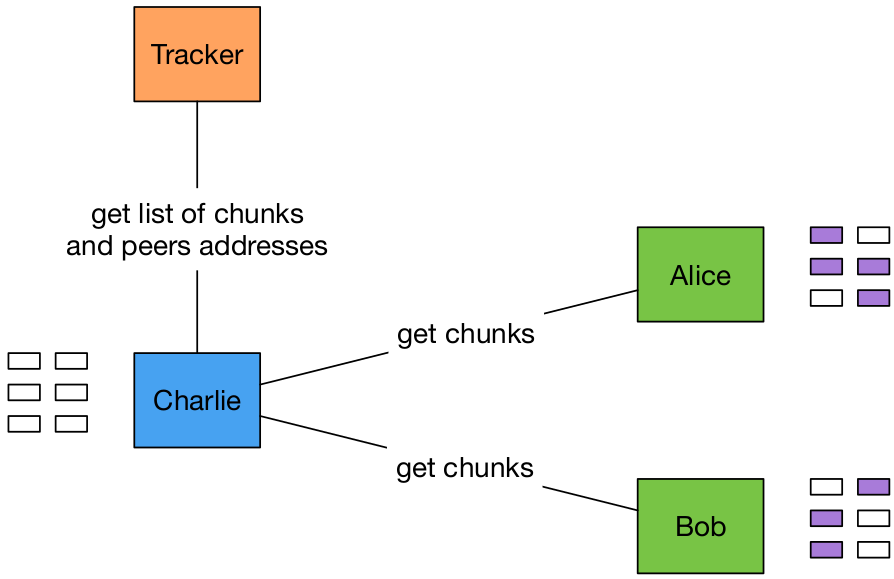
\includegraphics[width = 0.7\textwidth]{img/scheme.png}
    \caption{Scheme of the architecture}
    \label{fig:scheme}
\end{figure}

A file will be split in chunks, which will be distributed between the two peers. The client should be able to connect to the tracker in order to be informed of which peers owns which chunks, and then download the chunks and recover the original file.

The project is divided in three steps, the third one being optional. This report will, for each step, describe the objective of the step, present the description of the proposed solution and its particularities. Moreover, a sequence diagram will be provided.
